\documentclass[10pt,twocolumn,a4paper]{article}

% ------------------------------------------------------------------------------ Packages
\usepackage{amsmath}
\usepackage{color}
\usepackage{float}
\usepackage{graphicx}
\usepackage{lipsum}
\usepackage{listings}

% ------------------------------------------------------------------------------ Listing config
\definecolor{darkgreen}{rgb}{0,0.6,0}

\lstset{
    commentstyle=\color{darkgreen},
    keywordstyle=\color{blue},
    frame=single,
    language=C,
    breaklines=true,
    basicstyle=\tiny
}


% ------------------------------------------------------------------------------ Document begin
\begin{document}

% ------------------------------------------------------------------------------ Title
\title{CS499R: GPU Path Tracing}
\author{
    Student: Guillaume Abadie\\
    Professor: Stephen Mann
}
\date{\today}
\maketitle

% ------------------------------------------------------------------------------ Abstract
\begin{abstract}

Path tracing is a ray tracing based Monte Carlo rendering technic of images from
three-dimensional scenes, directly inspired from the modelisation of the light's
photons as rays going throught the scene. But instead of shooting the rays in the
same directection the photons would go, the Path Tracing is going the oposite
direction: From the camera to - hopefully - a light source. At every bounce, a new
ray is randomly regenerated to recursively continue the scene browsing for a
light source. Here is the reason why this technic stands as a Monte Carlo
algorithm: The rays we are shooting have chances - depending one the scene
being rendered - to not find any light source. One of main problem of this
technic is that it requires a hudge
amout of rays to be traced for a single pixel ray, so that the image's final
colors can converge thanks the low of large numbers. This memoire is the result
of a Path Tracer implementation
specifically designed to run on a GPU, in order to analyses differents
optimisations.

\end{abstract}

% ------------------------------------------------------------------------------ Introduction
\section{Introduction}
\subsection{Path tracer on a GPU}
Why would we like to implement a Path Tracer on a GPU rather than on a CPU?
The path tracing is shoting a lot of rays with a given random seed
for every pixel. Therefore the convenient thing is you can actually
compute two neighbouring pixels' color completly in parallel for instance.
Nowdays GPUs can run up to thousands threads in parrallel. And even GPU has
its own dedicated thread sheduling system that cam pause threads that are
waiting for a memory fetch for instance, giving the ALUs' compute power to
other thread waiting for available room to continue their execution. But also
this has some slight problems... Video memory is often around 2Gb. Not much if
we want to render a scene as detail as we would see in a movie today. But with
the GPU computing power increasing, considering a real-time path tracing with
simpler scene could very much make sense. This paper is then based in this
very last purpose.

\subsection{A paper dedicated for a GPU implementation}
Why a dedicated paper for Path Tracer implementations for GPU? This question is
can be awnsered with the following question: Why does the GPU has a much bigger
computing power than a CPU? GPUs and CPUs are both made same way:
integrated circuits scratched on wafers and then tiled out
into dies. But there differences come in the design of the transistors. The CPU
will be designed as a general purpose unit, that shall be the master of the
entire computer, giving orders and synchronising everything like a conductor
in an orchestre. Therefore, it needs to be able to do a lot of
different things, from managing the hardware interuptions to the wide range of
instruction set. On the otherhand, the GPU's cores are crowded on the die, thanks
to the fact that
they occupy a smaller size on the die. And since they occupy less space, they
can't do everything a CPU can. For instance, the instruction set of a GPU core
is basically restraint to memory
operations, arithmetic operations and few for logic/branching operations. Nothing else.
No hardware interuptions, no comunication with other component...

\subsection{Difference of a GPU implementation versus a CPU one}
What makes a Path Tracer implementation for GPU so different than for CPU? At
the begining, this project was only intended for studying memory corency on the
GPU, and memory access efficiency.
But it turned out that a bigger problem arises when it comes to a GPU
implementation: this what we will call in this paper the warp efficiency.

% ------------------------------------------------------------------------------ GPU background
\section{GPU background}
\subsection{Warp}
Given the number of cores and threads a GPU can run simultanously, the hardware
scheduler and all the compute unit would take a quite fair amout of space on the
die. So one major difference versus CPUs, is that GPUs core share a same
compute unit. The implementation might defer from the different constructor, but
the idea is ruffly the same. The threads are packed together in groups called
warps. Then each warp are scheduled on one of the existing compute unit, reading
only one stream of instructions for this warp and so gives ALU operation order
to the cores.

\subsection{Warp efficiency}
Originally, GPU thread were only used for dummy customatization at different
stages in the 3D rasterisation-based rendering pipeline like the following:
\begin{lstlisting}[morekeywords={vec3,texture}]
// GLSL fragment shader code of a normal maping
vec3 planNormal = texture(normalMap, uvCoord).xyz * 2.0 - 1.0;
vec3 meshNormal = tbnMatrix * planNormal;
vec3 lightColor = ambientLight + lightColor * dot(meshNormal, lightDirection);
vec3 meshAlbedo = texture(colorMap, uvCoord).rgb;
fragColor = meshAlbedo * lightColor;
\end{lstlisting}
So yes, we see that all threads would executes exactly the same instructions, so
packing them in warps is totally fine, removing transitors for the duplicated
compute unit that would just do the exact same sequences of states. But when
it comes to conditions and loops, required for an octree accelerated ray
intersection computation for instance, things are becoming tricky... Lets
consider the following code:
\begin{lstlisting}
if (/* condition */) {
    //operation A
}
else {
    //operation B
}
\end{lstlisting}
Remeber that a warp - a group of threads - are sharing the same compute unit. So
for a given warp, if all of its threads have the condition successing (or failing),
then the compute unit would only executes the operation A's instruction (respectively
operation B's instruction). So in those cases, this is completly fine. But in the
case of at least one thread would have a different condition result from its
brother in this given warp, then the compute unit would execute operation A's
instructions with a thread mask, and then operation B's instructions
with an inverted thread mask. It means that when a warp's compute unit is
executing instructions, some core might not be doing anything because of the
thread mask. So the warp efficiency over an execution is simply defined as:

\[\frac{\sum_{i \in instructions}activeThreads(i)}{| instructions | \times warpSize}\]

\subsection{Warp scheduling}
So both CPUs and GPUs have concept of threads. But the major difference between is
how the schedulers work. On the CPU, the sheduler is always a software scheduler
directly provided by the operating system. Mostly timer based preemptif
scheduler for a round-robin implementation, or a collatorative
sheduler where the applications yield its execution to another. But on modern GPU,
the sechduler is hardware based. You can not pause a GPU thread with an explicit
software call like pause().
But they are automatically paused and resumed by the hardware. Mostly on memory
operations, or a work group synchronisation barrier.

\subsection{Memory coherency}
As the CPUs, the GPUs also have memory caches. The memory is splitted into pages,
but only few of them can be stored in the nearby cache, and loading a page into
the cache is costly. Not many differences with a CPU, despite the fact that
their is going to have many more threads executing, making the cache access prediction
even tricky, and even impossible because of the warps' hardware scheduler running
on a quantum as small as memory fetch instruction.

\subsection{Memory access efficiency}
The convenient thing comes on memory operations. If you have very large scene, with a
lot of details, the memory coherency might drop completly, because clobered with
the many threads working at the same time. That means cache's page fault would become more frequent.
But this is where the warps' ahrdware scheduler come in. When a thread of a
warp wants to access a memory
location, it might take some time before it actually has the location's value.
So the hardware scheduler will then pause this warp, until the location's value
is available. Having paused this warp, the scheduler can then give another
warp to the newly available compute unit in the meantime. Therefore, on a GPU, we will
like to have even more threads than there is existing GPU cores to make sure the
hardware scheduler always have pending warp to give to the compute units, whereas
with a round robin software scheduler on a CPU, you would have many context
switches droping the computing efficiency.

% ------------------------------------------------------------------------------ Native implementation
\section{Native implementation}
\subsection{Octrees}
The testing implementation is using two octree layers. One for browsing the meshes
into the scene, and one for browsing triangles into the meshes. Both octree layers
uses sub-nodes reordering: access a node's sub-nodes in the order depending on
the direction of the ray, so that we can use the depth-test on nodes once we
have found a triangle intersection. We also enable back-face culling. Each octree
layer uses an iterative top to bottom browsing.

\subsection{Memory structure}
The common way to store data on GPU, is with array stored into buffers.
Our implementation uses 3 buffers:
\begin{description}
    \item[Octrees nodes' buffer] is the buffer that contain all octree nodes,
        from the scene's octree or the meshes' octree. A primitives (either a
        mesh or an instance) is only referenced into one octree node, to avoid
        primitive duplication or an index table.
        \begin{lstlisting}
struct octree_node_t
{
    // the sub-nodes' offset from the octree root
    uint32_t subnodeOffsets[8];
    // the first primitive (mesh or triangle) id
    uint32_t primFirst;
    // the number of primitives
    uint32_t primCount;
};
        \end{lstlisting}
    \item[Meshes instances' buffer] is the buffer containing all meshes intances.
        Each mesh instances contains information about the mesh to avoid an
        indirection into a mesh buffer.
    \item[Triangles' buffer] is the buffer containing all mesh's triangles
\end{description}
Some optimisations proposed below might modifies the structures.

\subsection{Tile and passes based rendering}
OpenCL commands must all have an constant upperbound running time, otherwise
you might trigger an GPU timeout that will kill your command. But computation
load is directly linked to the image size. In order to scale, we had to launch
our dispatch command per tile to guarentee that the image size doesn't affect
this timeout. Also, we wanted to changes our parameter for every pixel (MSA,
ray launched per pixel samples, recursions per rays...), so we also had to
render a tile with severals passes so it also doesn't affect the distpatch
command's execution time.

% ------------------------------------------------------------------------------ Warp efficiency optimizations
\section{Warp efficiency optimizations}
\subsection{Octree sub-nodes access lists}
\subsection{Octree tiny nodes pruning}
\subsection{Coherent Path Tracing}
\subsection{Coherent Interleaved Path Tracing}
\subsection{Coherent Path Tracing Super sampling}
\subsection{Octree one loop browsing}
As said above, our implementation uses 2 octree layers: one for the scene browsing,
and one for the meshes' browsing. Thats means the algorithm uses nested loops.
\begin{figure}[H]
    \centering
\begin{lstlisting}[morekeywords={foreach}]
foreach intersected node in the scene octree
{ // loop 1
  foreach mesh in this scene node
  { // loop 2
    foreach intersected node in mesh s octree
    { // loop 3
      foreach triangle in this mesh node
      {
        intersect_triangle();
      }
    }
  }
}
\end{lstlisting}
    \caption{Octree layers' browsing loops}
    \label{code:octree_layers_loops}
\end{figure}

Therefore, the problem is when we are coming to very detailed meshes, some thread
of a same warp might have less loop~3's iterations in loop~1's first iterations,
but more loop~3's iterations in loop~1's second iterations for instance. But since
there are executed in the same warp, all loop will be synchronized. Meaning all
loop shall finish at the same time. The idea of this optimization
is to collapses loop~1, 2 and 3 as shown on Figure~\ref{code:octree_layers_loops}
by an one loop based state machine.

\begin{figure}[h]
    \centering
    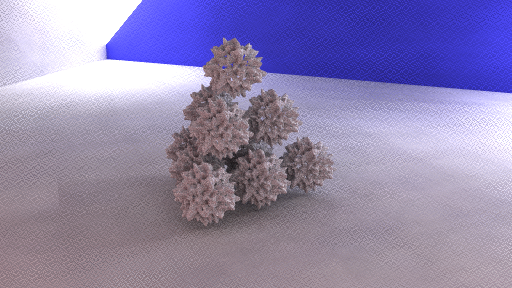
\includegraphics[width=0.8\columnwidth]{render_displaced_spheres.png}
    \caption{Displaced spheres}
    \label{fig:displaced_spheres}
\end{figure}

\begin{figure}[h]
    \centering
    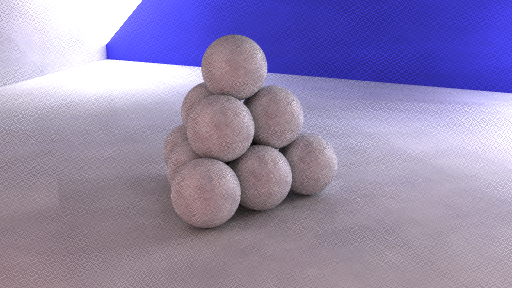
\includegraphics[width=0.8\columnwidth]{render_spheres.png}
    \caption{Simple spheres}
    \label{fig:spheres}
\end{figure}

\begin{figure}[H]
    \tiny
    \centering
    \begin{tabular}{ | l | c | c | }

        \hline
        Octree one loop & Simple spheres & Displaced spheres \\
        \hline
        Disabled & 374.2ns & 1746.9ns \\
        Enabled & 410.1ns & 1522.2ns \\
        \hline

    \end{tabular}
    \caption{Octree one loop browsing's average rendering time per ray}
    \label{table:octree_one_loop_browsing}
\end{figure}

We can actually witness on Figure~\ref{table:octree_one_loop_browsing} that
there is a rendering time improvement on a scene having nearby detailed meshes
(as Figure~\ref{fig:displaced_spheres} shows), thanks to the removal of the warp's thread
synchronisation caused by the nested loops, improving the warp efficiency. But
when rendering scene having non-detailed meshes (as Figure~\ref{fig:spheres} shows), we
are witnessing a performance drop, caused by the states-machine's conditions
overload.


% ------------------------------------------------------------------------------ Memory coherency optimizations
\section{Memory coherency optimizations}
\subsection{Octree consecutives sub-nodes}


% ------------------------------------------------------------------------------ Appendix
%\appendix

\end{document}
